%% Springer Nature LaTeX template (sn-jnl) -- NLP course final project
%% Adapted from the official sn-article.tex demo. The original demo file is
%% preserved as sn-article_DEMO-original.tex.bak in this folder.
%%
%%%%%%%%%%%%%%%%%%%%%%%%%%%%%%%%%%%%%%%%%%%%%%%%%%%%%%%%%%%%%%%%%%%%%%
%%                                                                 %%
%% Please do not use \input{...} to include other tex files.       %%
%% Submit your LaTeX manuscript as one .tex document.              %%
%%                                                                 %%
%%%%%%%%%%%%%%%%%%%%%%%%%%%%%%%%%%%%%%%%%%%%%%%%%%%%%%%%%%%%%%%%%%%%%

\documentclass[pdflatex,sn-mathphys-num]{sn-jnl}% Math and Physical Sciences Numbered Reference Style

%%%% Standard Packages
\usepackage{graphicx}%
\usepackage{multirow}%
\usepackage{amsmath,amssymb,amsfonts}%
\usepackage{amsthm}%
\usepackage{mathrsfs}%
\usepackage[title]{appendix}%
\usepackage{xcolor}%
\usepackage{textcomp}%
\usepackage{booktabs}%
%%%%

\graphicspath{{figures/}}

\theoremstyle{thmstyleone}%
\newtheorem{theorem}{Theorem}%
\newtheorem{proposition}[theorem]{Proposition}%
\theoremstyle{thmstyletwo}%
\newtheorem{example}{Example}%
\newtheorem{remark}{Remark}%
\theoremstyle{thmstylethree}%
\newtheorem{definition}{Definition}%

\raggedbottom

\begin{document}

\title[Reasoning, Adaptation, or Imitation in LLM Negotiation]{Reasoning, Adaptation, or Imitation? A Three-Lens Analysis of Emergent Strategy in LLM Negotiation Agents}

\author*{\fnm{Alessandro} \sur{Bottoni}}\email{alessandrobottoni.ab@gmail.com}

\abstract{When two large language model (LLM) agents negotiate, they produce behaviour that \emph{looks} strategic --- probing, framing, concession, strategic disclosure --- but it is unclear whether this reflects genuine, situation-specific reasoning, pragmatic adaptation to the dialogue, or scripted imitation of prompt patterns. We place buyer and seller agents, built on DeepSeek-R1 (which exposes its private chain-of-thought through a dedicated API field), in a software sale with a deliberate information asymmetry: the seller secretly knows the product has a critical bug. Across four persona configurations (160 negotiations) we compare a zero-shot baseline with a prompt-based behavioural-cloning condition in which an Observer agent reinjects the most successful tactics into the agents' prompts. The contribution is a three-lens framework that operationalises imitation, adaptation, and reasoning with reproducible metrics rather than treating ``good negotiation'' as one undifferentiated quantity. The central finding is a clarifying trade-off: cloning makes the agents far more effective --- agreement rises from 70\% to 100\% and deals close in roughly half the turns, with prices collapsing toward the seller's floor --- yet the chain-of-thought analysis shows this efficiency is bought by a shift away from contingent, dialogue-anchored reasoning toward directive, script-following reasoning, a distinction outcome metrics alone would conflate.}

\keywords{Large language models, multi-agent negotiation, chain-of-thought, social learning, behavioural cloning}

\maketitle

\section{Introduction}\label{sec:intro}

Negotiation is one of the richest testbeds for studying communicative intelligence: an agent must pursue a private objective, model its counterpart, manage incomplete information, and adapt as the dialogue unfolds. With LLMs now capable of fluent, open-ended dialogue, two such models can be placed in opposition and observed as strategies emerge --- persuasion, concession, framing, strategic disclosure, even deception --- without any being hand-coded. This raises a question both scientifically interesting and practically consequential: when an LLM agent \emph{appears} to negotiate skilfully, what is happening underneath? Is it reasoning about the specific situation, or reproducing surface patterns absorbed from its prompt?

Lewis et al.\ \cite{lewis2017} showed that neural models trained end-to-end on a bargaining task can negotiate in natural language and even learn to deceive; we inherit their premise but shift the emphasis from optimising outcomes to understanding what kind of competence underlies skilled-looking behaviour. A second strand studies how behaviour changes when LLM agents learn from successful peers \cite{gupta2025}, motivating our comparative design. The enabling ingredient is the model: DeepSeek-R1 \cite{deepseekr1} returns its chain-of-thought (CoT) in a dedicated \texttt{reasoning\_content} field, separate from the message it sends, letting us log each agent's \emph{private} reasoning per turn and ask whether it is genuinely tied to the negotiation.

The contribution is a \textbf{three-lens framework} that distinguishes three explanations for skilled-looking behaviour --- \emph{scripted imitation}, \emph{pragmatic adaptation}, and \emph{genuine reasoning} --- and operationalises each with reproducible metrics. We exercise it with a two-phase design: a zero-shot baseline, then a lightweight, prompt-based form of social learning. Comparing the phases reveals not just \emph{whether} behaviour improves but \emph{which} lens accounts for the change. In keeping with the project brief, the emphasis is not on maximising performance but on a critical reading of what the methodology can reveal.

\section{Research Question and Methodology}\label{sec:method}

\subsection{Research question}\label{subsec:rq}

We investigate one central question: \emph{what communicative strategies emerge when LLM agents negotiate over multiple rounds, and to what extent they transition from pattern imitation to deeper strategic choices?} We operationalise it along three axes that form the analytical core of the work: \textbf{scripted imitation} (reproducing prompt/few-shot patterns with little adaptation), \textbf{pragmatic adaptation} (applying a tactic but modulating it to the dialogue state), and \textbf{genuine reasoning} (structured, conditional reasoning that integrates dialogue history and yields strategies not present in the prompt).

\subsection{Scenario and personas}\label{subsec:scenario}

The negotiation is a \textbf{software sale with information asymmetry}. The \emph{seller} privately knows the product has a critical bug; its goal is to maximise price and it is told not to disclose the bug spontaneously. The \emph{buyer} has a \texteuro10{,}000 budget and aims to minimise price and avoid risk, probing for hidden problems. The bug is a natural pivot for strategies such as bluffing, omission, probing, and strategic disclosure. Agent disposition is varied through three persona archetypes (Table~\ref{tab:personas}) combined into four role configurations. A--C hold the seller constant and vary the buyer, isolating buyer type; D reverses roles to test whether patterns are driven by persona or by negotiation role.

\begin{table}[tb]
\caption{Persona archetypes (left) and the four role configurations (right; $\sim$20 negotiations per cell per phase).}\label{tab:personas}\label{tab:configs}
\centering
\begin{tabular}{@{}l@{\hspace{3em}}l@{}}
\begin{tabular}[t]{@{}lp{0.34\textwidth}@{}}
\toprule
Persona & Goal / characteristic behaviour \\
\midrule
Maximiser & Maximise own utility; aggressive, withholds information, applies pressure \\
Fairness-seeker & Reach a fair outcome; transparent, concedes, resists deception \\
Risk-minimiser & Avoid bad outcomes; cautious, asks many questions \\
\botrule
\end{tabular}
&
\begin{tabular}[t]{@{}ccc@{}}
\toprule
Cfg & Seller & Buyer \\
\midrule
A & Max & Max \\
B & Max & Risk \\
C & Max & Fair \\
D & Fair & Max \\
\botrule
\end{tabular}
\end{tabular}
\end{table}

\subsection{Model and the private chain-of-thought}\label{subsec:model}

All agents use DeepSeek-R1 \cite{deepseekr1}, whose API returns the CoT in a \texttt{reasoning\_content} field, separate from the \texttt{content} sent to the counterpart. The loop logs the CoT \emph{before} forwarding only the message --- a ``private thought'' mechanism obtained without any architectural change. OpenAI o-series models were rejected because their reasoning tokens are never exposed, which would make the genuine-reasoning lens intractable. This single capability is load-bearing, and we revisit its limits in Section~\ref{sec:conclusion}.

\subsection{Two-phase design}\label{subsec:phases}

In \textbf{Phase 1} each configuration runs $\sim$20 zero-shot negotiations (80 total), iterating until a firm agreement or impasse (16-turn cap), logging the transcript, per-turn CoT, outcome and price, bug disclosure/discovery, and turn count. Firm decisions use a structured agent-emitted tag (\texttt{[DEAL: <price>]} / \texttt{[NO DEAL]}), after an earlier keyword detector proved brittle to deal-related words in non-conclusive contexts. \textbf{Phase 2} implements social learning and behavioural cloning purely through prompts. A third DeepSeek-R1 instance acts as an \emph{Observer}: it scores each agent's performance on a 1--5 scale, receiving the full transcript together with the scenario description and both persona labels but no explicit rubric --- scoring criteria are implicit, with the model expected to infer what counts as good performance from persona and context (e.g.\ a Maximiser seller should maximise price) and required to supply a written rationale for each score. The one or two top-scoring sessions per role are then selected and the Observer extracts an abstract tactic description plus representative snippets, injected into the agents' prompts as few-shot guidance; the same 80 negotiations are re-run. We use ``behavioural cloning'' and ``social learning'' in an extended, prompt-engineering sense rather than their gradient-based definitions, justified by the functional analogy: agents learn from successful peers and update their behaviour.

\subsection{Operationalising the three lenses}\label{subsec:metrics}

Each lens is tied to a concrete measure computed offline. \emph{Scripted imitation} is the sentence-embedding cosine similarity (\texttt{all-MiniLM-L6-v2} \cite{reimers2019}) between a Phase 2 agent's turns and the few-shot example in its prompt; the threshold of $0.75$ was fixed by manually labelling a stratified sample and choosing the value that best separates imitation from adaptation. \emph{Pragmatic adaptation} is scored per turn by an independent LLM-judge on a $1$--$3$ scale ($1=$ rigid, $3=$ adaptive and tailored). \emph{Genuine reasoning} is assessed \emph{per turn}, so we can test whether the reasoning at turn $N$ responds to the dialogue visible up to turn $N{-}1$. We extract \emph{anchor tokens} from the visible transcript (prices, percentages, content-related words $\geq 4$ characters, excluding a list of stop-words defined by analysing a few conversation samples) and define the \textbf{grounding score}
\begin{equation}
g_N = \frac{|\,A^{\mathrm{cot}}_N \cap A^{\mathrm{dlg}}_{<N}\,|}{|\,A^{\mathrm{dlg}}_{<N}\,|},\label{eq:grounding}
\end{equation}
the fraction of available dialogue anchors $A^{\mathrm{dlg}}_{<N}$ that reappear in the turn-$N$ CoT: a generic CoT such as ``maximise price'' cites at most two anchor tokens against the full pool accumulated in the dialogue history, yielding a score near zero; one citing ``their 6500 offer, which undercuts my 7000 floor'' references several dialogue-specific anchors --- \texttt{6500}, \texttt{offer}, \texttt{7000}, \texttt{floor} --- and scores substantially higher. \textbf{Conditional specificity} is computed per turn as the fraction of conditional clauses (``if'', ``otherwise'') in the CoT that contain at least one anchor --- a turn raising no conditional scoring zero --- and reported as the mean across turns; it thus rewards reasoning that is both \emph{contingent} and dialogue-anchored while penalising generic hedging as well as the mere absence of contingent deliberation. At Level 2, an auxiliary classifier rates each CoT on \emph{context specificity} (generic vs.\ dialogue-specific) and \emph{planning depth} (immediate vs.\ multi-branch) on $1$--$3$ scales, an independent check on the offline metrics.

\section{Experimental Results}\label{sec:results}

\subsection{Corpus and quantitative outcomes}\label{subsec:quant}

The corpus is fully synthetic: 160 negotiations, each a structured record with the visible transcript, per-turn private CoT, and outcome metadata. The phases differ sharply in size despite the identical session count --- an early signal of the behavioural shift below: Phase 1 has $759$ messages ($\approx$42{,}800 words), Phase 2 only $367$ ($\approx$26{,}100 words). After social learning, agents agree using a little under half as many messages while writing longer individual ones.

Table~\ref{tab:quant} aggregates the per-configuration statistics; Figure~\ref{fig:outcomes} shows the two headline movements. The clearest is configuration B's jump in agreement from $0.15$ to $1.00$: the learned tactics resolve precisely the impasse a cautious, walk-away-prone buyer could not get past against an aggressive seller. Prices, both higher and far more dispersed in Phase 1, collapse toward the seller's \texteuro7{,}000 reservation in Phase 2, and their variance shrinks (configuration C settles at exactly \texteuro7{,}500). B makes the trade-off starkest: agreement reaches 100\% but the mean price falls from \texteuro9{,}500 to \texteuro7{,}235 --- a reliable close bought by leaving roughly \texteuro2{,}265 on the table. Negotiations also close much faster (mean turns $\approx$8 $\rightarrow$ $\approx$3.5). Bug disclosure and discovery were already near-ceiling in Phase 1 and uniform in Phase 2 (detection is keyword-based, so these rates mean ``the topic surfaced'' rather than a semantic judgement; see Section~\ref{sec:conclusion}).

\begin{table}[tb]
\caption{Aggregated outcomes per configuration and phase.}\label{tab:quant}
\begin{tabular*}{\textwidth}{@{\extracolsep\fill}cccccc@{}}
\toprule
Config & Phase & Agreement & Mean price (\texteuro) & Std price & Mean turns \\
\midrule
A & 1 & 0.70 & 7{,}750 & 849.2 & 7.90 \\
A & 2 & 1.00 & 7{,}085 & 184.3 & 3.90 \\
B & 1 & 0.15 & 9{,}500 & 866.0 & 8.80 \\
B & 2 & 1.00 & 7{,}235 & 249.8 & 3.65 \\
C & 1 & 1.00 & 9{,}455 & 532.6 & 8.60 \\
C & 2 & 1.00 & 7{,}500 & \phantom{0}\,\,0.0 & 2.90 \\
D & 1 & 0.95 & 7{,}105 & 267.7 & 8.65 \\
D & 2 & 1.00 & 7{,}200 & 251.3 & 3.90 \\
\botrule
\end{tabular*}
\end{table}

\begin{figure}[tb]
\centering
\begin{minipage}[c]{0.45\linewidth}\centering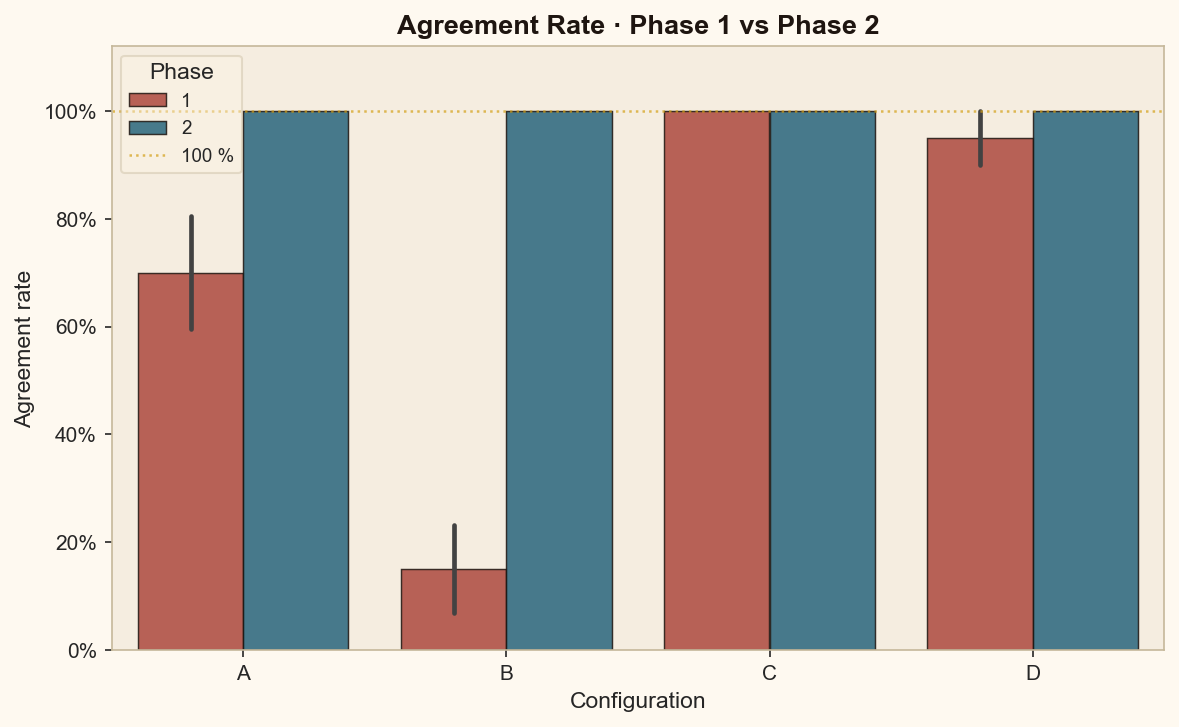
\includegraphics[width=\linewidth]{agreement_rate.png}\end{minipage}\hfill
\begin{minipage}[c]{0.45\linewidth}\centering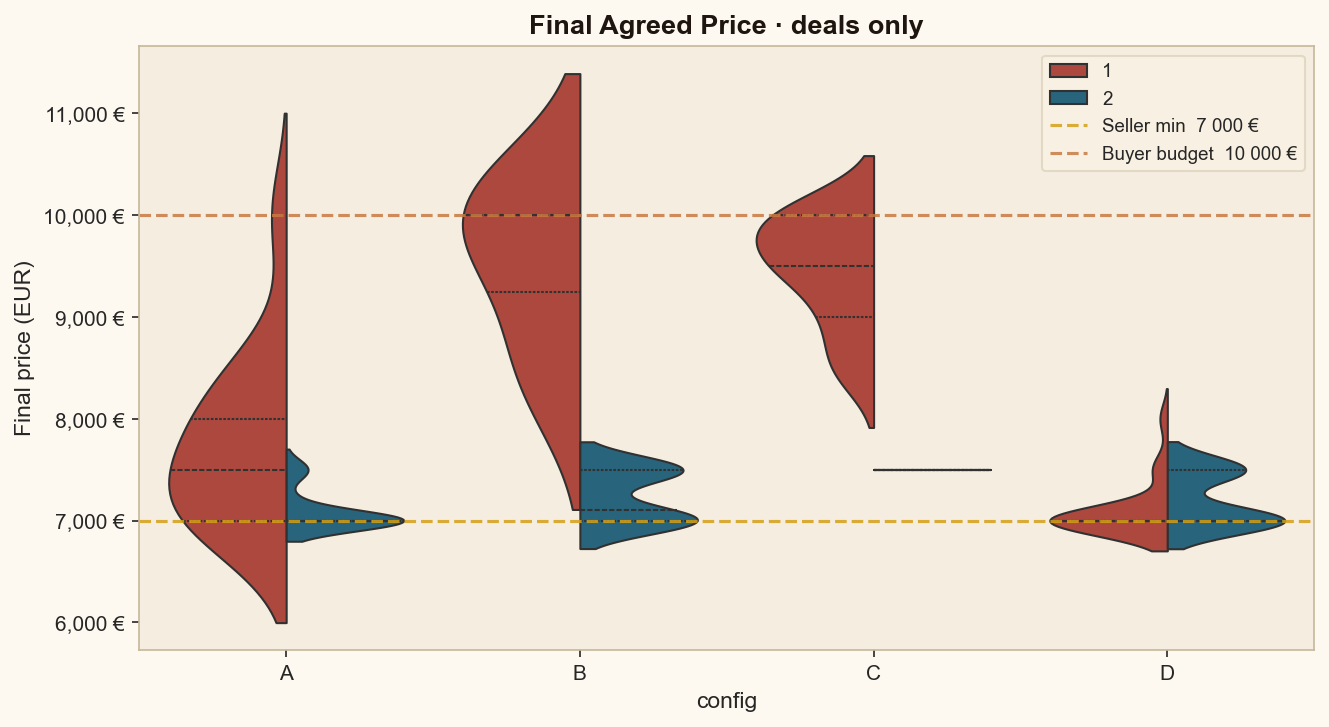
\includegraphics[width=\linewidth]{price_distribution.png}\end{minipage}
\caption{\textbf{Outcomes.} \emph{Left:} agreement rate --- the baseline depends heavily on the persona pairing (configuration B closes only 15\% of the time), whereas after social learning every configuration reaches 100\%. \emph{Right:} final agreed prices (deals only, Phase~1); in Phase~2 prices collapse toward the seller's \texteuro7{,}000 floor.}\label{fig:outcomes}
\end{figure}

\subsection{The three lenses}\label{subsec:lenses}

Read through the framework, the lenses point in different directions.

\textbf{Pragmatic adaptation.} The LLM-judge's mean appropriateness rises from $\approx$2.65 to $\approx$2.96 (Figure~\ref{fig:level}, left). In the baseline, adversarial pairings score lowest (A 2.32, B 2.44) while those with a Fairness-seeker score highest; after cloning every configuration sits near the ceiling. On this lens Phase 2 is unambiguously \emph{better}.

\textbf{Scripted imitation.} Mean cosine similarities cluster tightly at or just above the calibrated $0.75$ threshold ($0.750$--$0.765$). Sitting on the boundary, the evidence is genuinely mixed: agents neither slavishly copy nor fully depart from the injected examples --- they reuse the gist while varying the surface form. A caveat from calibration: cosine similarity captures \emph{semantic} proximity but not verbatim \emph{lexical} copying, so a complementary n-gram measure would sharpen this lens.

\textbf{Genuine reasoning.} The per-turn CoT analysis is where the framework earns its keep, with a partly counter-intuitive result. The grounding score (Figure~\ref{fig:cot}, left) spikes at turn~1 to $\approx$0.30 in Phase 2, double the Phase 1 value: primed with a tactic, the Phase 2 buyer immediately references the anchors the seller just introduced, whereas the zero-shot buyer is vaguer --- the cleanest evidence that cloning ``works''. Yet conditional specificity (Figure~\ref{fig:cot}, right) is \emph{higher} in Phase 1 than Phase 2 in all four configurations (C collapses from $0.37$ to $0.08$). The interpretation is coherent: lacking a prescribed tactic, baseline agents reason contingently (``if they accept I concede, otherwise I hold firm''), and those conditionals cite concrete anchors; once the tactic is supplied, reasoning becomes directive (``execute the planned move'') and the surviving conditionals are mostly unanchored boilerplate (``if I push too hard''). The Level-2 classifier corroborates this independently: context specificity edges down ($2.20 \rightarrow 2.16$) while planning depth stays uniformly low ($\approx$1.61 in both phases). On the per-session scatter (Figure~\ref{fig:level}, right) most sessions fall in the moderate-specificity, low-planning region rather than the high/high ``genuine-reasoning'' quadrant --- explicit multi-branch planning is rare under either condition.

\begin{figure}[tb]
\centering
\begin{minipage}[c]{0.45\linewidth}\centering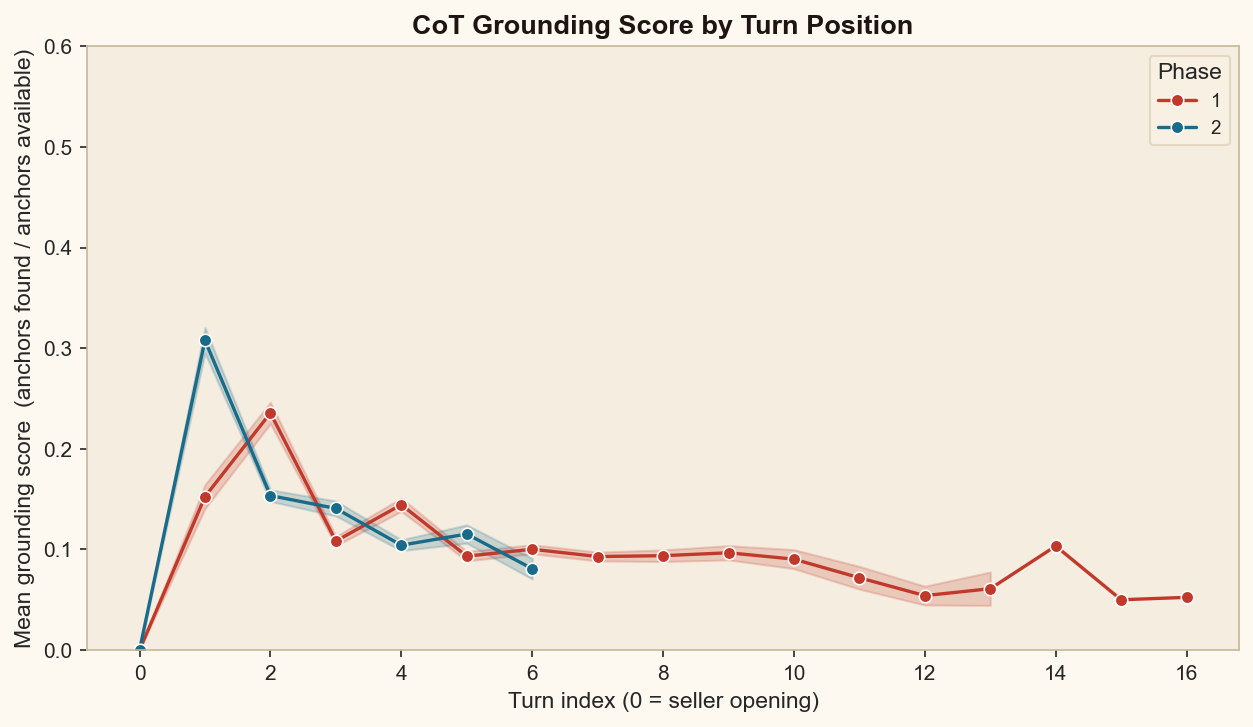
\includegraphics[width=\linewidth]{cot_grounding_by_turn.png}\end{minipage}\hfill
\begin{minipage}[c]{0.45\linewidth}\centering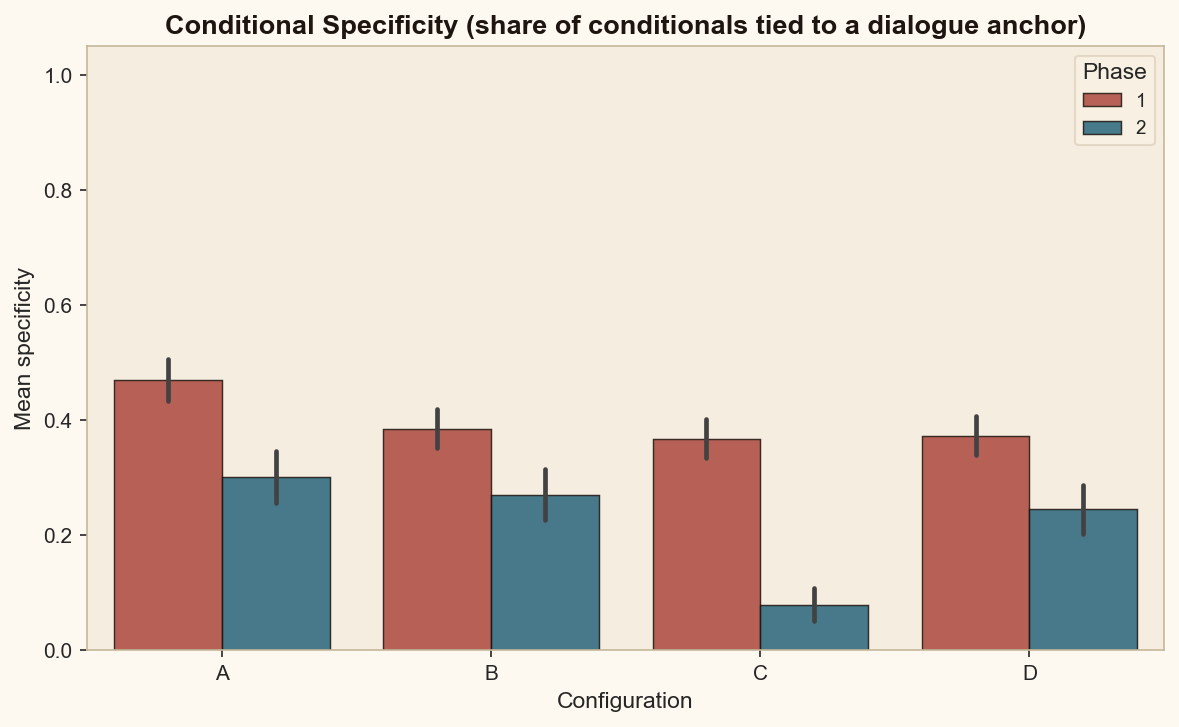
\includegraphics[width=\linewidth]{cot_conditional_specificity.png}\end{minipage}
\caption{\textbf{Genuine-reasoning lens.} \emph{Left:} grounding score (Eq.~\ref{eq:grounding}) by turn position --- Phase 2 grounds twice as strongly at turn~1, then crosses below Phase~1; the slow later decline is partly a mechanical artefact (the anchor denominator grows cumulatively), so interpretation concentrates on the first three turns. \emph{Right:} conditional specificity --- contingent, anchored reasoning is \emph{lower} in Phase~2 across all four configurations, the central qualitative finding.}\label{fig:cot}
\end{figure}

\begin{figure}[tb]
\centering
\begin{minipage}[c]{0.45\linewidth}\centering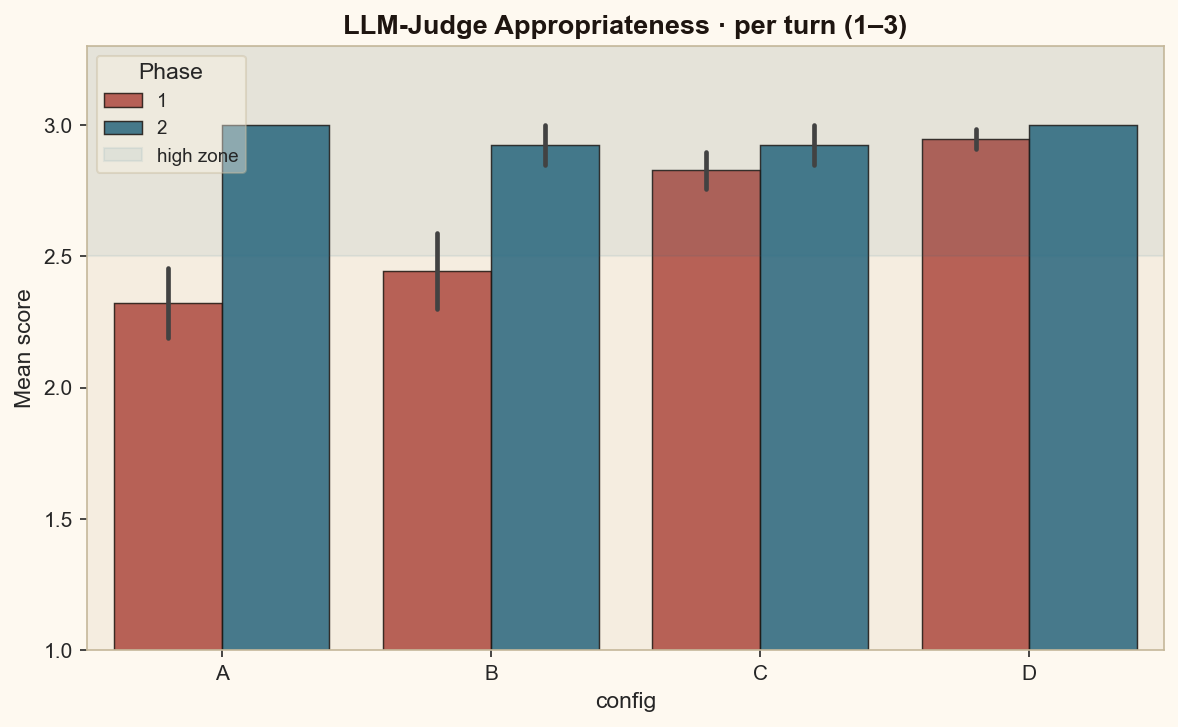
\includegraphics[width=\linewidth]{llm_judge.png}\end{minipage}\hfill
\begin{minipage}[c]{0.45\linewidth}\centering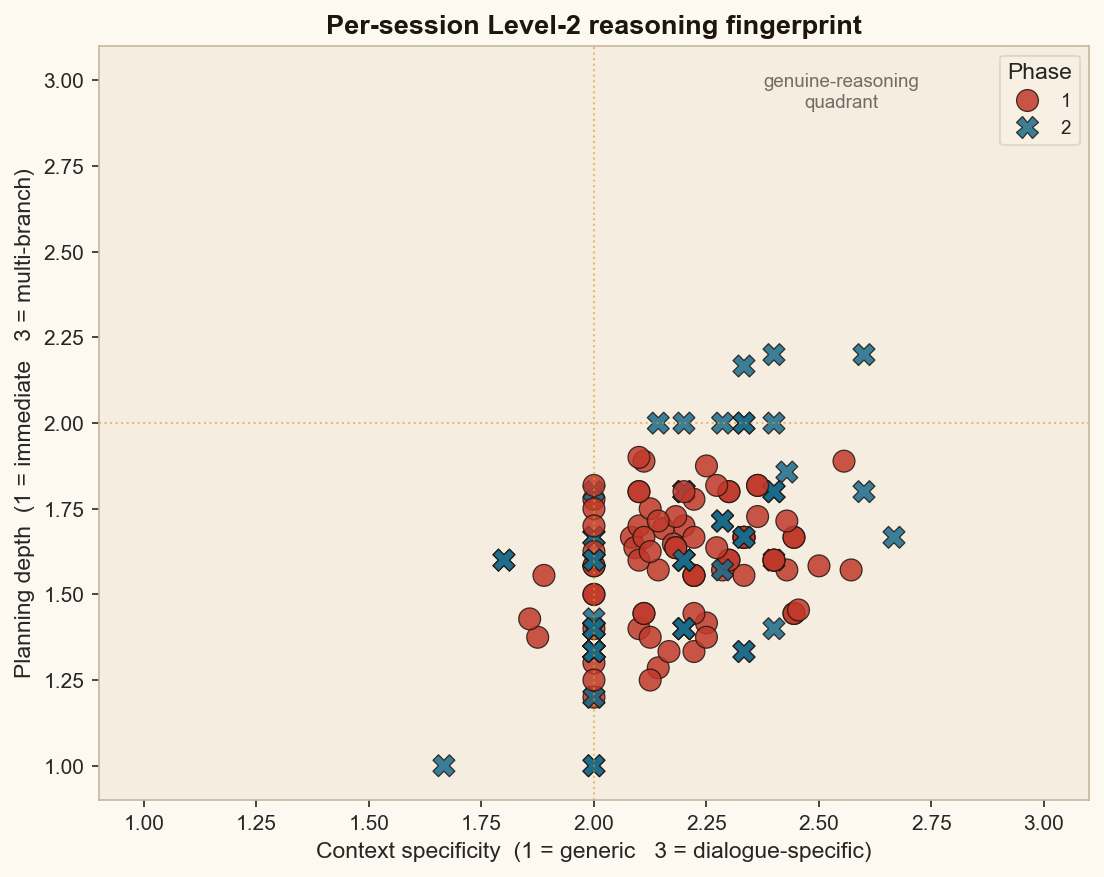
\includegraphics[width=\linewidth]{cot_llm_scatter.png}\end{minipage}
\caption{\textbf{Adaptation and Level-2 reasoning.} \emph{Left:} LLM-judge per-turn appropriateness; social learning raises every configuration into the ``high'' zone, with the largest gains on the adversarial pairings. \emph{Right:} per-session means of context specificity vs.\ planning depth; both phases cluster away from the genuine-reasoning quadrant, with planning depth staying low.}\label{fig:level}
\end{figure}

\textbf{What the agents actually do.} The two injected tactics are structurally complementary, which explains the convergence: the winning \emph{seller} tactic is \textbf{proactive framed disclosure} (surface the defect early in a remediation frame, pre-empting the buyer's discovery and justifying a pre-packaged concession), and the winning \emph{buyer} tactic is \textbf{probing plus a risk-anchored offer} (interrogate for documented issues, then re-anchor the valuation low once a defect is confirmed). Because disclosure anticipates the probe, both reach the bug juncture faster and the negotiation collapses to three or four turns. A manual scan confirms most Phase 2 transcripts follow this playbook closely; the few novel moves appear almost exclusively in longer-than-average sessions, where the injected script runs out of prescriptions --- consistent with the conditional-specificity finding.

\textbf{Synthesis.} Phase 2 improves on \emph{pragmatic adaptation} (100\% agreement, higher judge score) and reuses the injected examples enough to register as partial \emph{scripted imitation} (similarity at the threshold), but shows a modest reduction in the structural correlates of \emph{genuine reasoning} (lower conditional specificity, lower Level-2 specificity, a flatter effort profile). Efficiency and reliability are purchased at the cost of contingent deliberation.

\section{Concluding Remarks}\label{sec:conclusion}

\textbf{Critical discussion.} The study asked not merely \emph{whether} LLM agents negotiate well but \emph{what kind} of competence underlies their behaviour, and the salient result is a trade-off surfaced by the framework rather than by any single metric. Prompt-based behavioural cloning makes the agents demonstrably more effective --- agreement rises from 70\% to 100\%, deals close in roughly half the turns, and prices converge toward the seller's reservation --- so an evaluation reading only these numbers would record an unambiguous success. The chain-of-thought lens is more cautionary: the same intervention shifts agents \emph{away} from contingent, dialogue-anchored reasoning toward directive, script-following reasoning --- they latch onto context faster (higher grounding at the first move) but deliberate less conditionally (lower conditional specificity in every configuration, corroborated by the Level-2 classifier). The single interpretation is that \textbf{prompt-based social learning buys efficiency and reliability at the cost of some genuine, contingent reasoning}, replacing context-dependent deliberation with a pre-validated, standardised script. This is not a defect of the method but a clarifying observation about what ``social learning via prompting'' does to an agent's internal process. Crucially, outcome metrics conflate this effect; only the combination of lenses --- enabled by access to the private chain-of-thought --- makes it visible, separating ``the agents got better'' from ``the agents got better \emph{at the same thing}''.

\textbf{Limitations.} Several caveats apply. The study is \emph{single-model dependent}: the reasoning analysis is only possible because DeepSeek-R1 exposes its CoT, but that CoT is a \emph{rationalisation produced by the model}, not a guaranteed faithful trace, and findings may not transfer across model families. There is \emph{LLM-evaluating-LLM circularity} --- the Observer, judge, and Level-2 classifier are themselves LLMs, and only the cosine-similarity threshold received human verification, so judge and classifier outputs are indicative; additionally, the Observer's scoring rubric is implicit (no explicit criteria were provided), so the selection of ``top'' sessions is model-dependent and may not align with a human analyst's judgement of success. \emph{Bug detection is keyword-based}, measuring whether the topic surfaced rather than making a semantic judgement, with broad triggers inflating near-ceiling rates. The \emph{grounding score} has a cumulative denominator (Eq.~\ref{eq:grounding}), making the cross-turn decline partly mechanical. Finally, \emph{scope} is limited: one scenario, one model, four pairings, and 20 sessions per cell, with no out-of-distribution perturbation tests.

\textbf{Future work.} The most direct extension is \textbf{gradient-based behavioural cloning} via LoRA fine-tuning on an open-weight model, trained on the Phase 1 demonstrations, enabling a clean comparison with the prompt-based variant. \textbf{Out-of-distribution perturbation tests} (different product, bug type, price range, or time pressure) would sharpen the imitation/adaptation distinction. Other directions include a \textbf{recency-weighted grounding score} correcting the cumulative-denominator artefact, a \textbf{semantic bug-disclosure classifier} replacing the keyword flags, and a human-in-the-loop variant.

\backmatter

\section*{Declarations}

\bmhead{Data and code availability} All evaluation logic is implemented as importable Python modules; the figures and aggregated tables are produced offline from the logged JSON transcripts.

\bmhead{AI usage disclaimer} The following AI assistants were used: Claude (Anthropic) and Gemini (Google), for brainstorming research directions and experimental design; writing, debugging, and reviewing code; locating and summarising relevant papers; supporting the project architecture; and drafting and editing sections of this report. All research questions, experimental choices, analytical interpretations, and conclusions are the author's own. AI-generated code was read, tested, and validated before use, and AI-generated prose was reviewed and edited by the author, who retains full responsibility for the content, reasoning, and conclusions of this work.

\bibliography{sn-bibliography}%

\end{document}
